\documentclass[10pt]{beamer}
\usepackage{listings}
\usepackage[utf8]{inputenc}
\usefonttheme{structuresmallcapsserif}
\usetheme{Madrid}

\usepackage{color}

\definecolor{lightgrey}{rgb}{0.9,0.9,0.9} % defining color for listing
\definecolor{darkgreen}{rgb}{0,0.6,0} % defining color for listing

\lstset{language=[LaTeX]TeX,
texcsstyle=*\bf\color{blue},
numbers=left,
breaklines=true,
keywordstyle=\color{darkgreen},
commentstyle=\color{red},
morekeywords={},
otherkeywords={$,\{ ,\} , [ , ] },
frame=leftline,
tabsize=2,
backgroundcolor=\color{lightgrey},
%escapeinside=||
}


\begin{document}

\title{An Introduction to fold}   
\author{Pavel Paroulek}  
\date{\today} 

\frame{\titlepage} 


\section{Section no. 0} 
\subsection{Lists I}
\frame{\frametitle{About explicit recursion}
\begin{itemize}
\item Explicit recursion in FP is harder to read and reason about  
\item Some consider it a \textit{goto} statement in the FP world
\item One can avoid it with more structured aproaches to recursion
\item Usually higher order functions that 'abstract-away' recursion statements
\item Possibility to take advantage of laws and properties which these abstraction conform to
\end{itemize}
\begin{block}{xkcd 292 - goto}
\includegraphics[width=\textwidth]{goto.png}
\end{block}}


\section{Section no. 0} 
\subsection{Lists I}
\begin{frame}[fragile]
\frametitle{Example of higher order function}
\begin{itemize}
\item Some useful functions in FP: map, filter, zipWith, \textbf{fold}, unfold ...
\item zipWith $:: (a \rightarrow b \rightarrow c) \rightarrow [a] \rightarrow [b] \rightarrow [c]$
\item Example - sum of elements at the same position in $[1,1,1]$ and $[1,2,3]$
\item Result should be $[1+1, 1+2,1+3]$ (i.e. $[2,3,4]$) 
\end{itemize}

\begin{lstlisting}
count [] [] = 0
count (x:xs) (y:ys) = x + y + (count xs ys) 

\end{lstlisting}


\begin{itemize}
\item We can use the function $zipWith$ 
\end{itemize}
\begin{lstlisting}
let l1 = [1,1,1] 
let l2 = [1,2,3] 
count l1 l2 == [2,3,4] // True	
zipWith (+) l1 l2 == count l1 l2 // True 	

\end{lstlisting}
\end{frame}


\begin{frame}[fragile]
\frametitle{fold as a powerful higher order function}
\begin{itemize}
\item \textit{fold} is a structured way to go over lists  	
\item It reduces/processes the input list applying a given function
\item The signature is $(a \rightarrow b \rightarrow a) \rightarrow  a \rightarrow  [b] \rightarrow a$ where the first argument is a
	function, second argument is a initial value of the accumulator and the third value the list being processed
\item Through fold one can define other higher order functions like length, map, filter, reverse, sum ...
\end{itemize}

\begin{lstlisting}
map :: (a -> b) -> [a] -> [b]
map f = foldl (\xs x -> xs ++ [f x]) [] 
map (+1) [1,2,3] == [2,3,4] //True
\end{lstlisting}

\end{frame}


\begin{frame}[fragile]
\frametitle{Properties of fold}
\begin{itemize}
\item There are certain properties, that have been derived for fold 
\item The properties apply generally for folds on lists 
\item The 'universal property' implies that if you have the following idiom   	
\end{itemize}

\begin{lstlisting}
h []     = v
h (x:xs) = f x (h xs)
\end{lstlisting}

\begin{itemize}
\item it is possible to replace it with
\end{itemize}

\begin{lstlisting}
h = fold f v
\end{lstlisting}

\end{frame}



\begin{frame}[fragile]
\frametitle{Example of the Universal property}
\begin{itemize}
\item Let's rewrite the filter function as a fold using the universal property
\item Based on a given function filter removes certain elements from the input list 	
\item 'h (x:xs) = f x (h xs)'
\end{itemize}

\begin{lstlisting}
filter :: (a -> Bool) -> [a] -> [a]
filter g  [] = []
filter g (x:xs)  
    | g x       = x : filter g xs 
    | otherwise = filter g xs
\end{lstlisting}

\begin{itemize}
\item in this case f could have the form f x xs = IF condition THEN recursive\_op1 ELSE recursive\_op2 
\end{itemize}

\end{frame}






\begin{frame}[fragile]
\frametitle{Example of the Universal property}
\begin{itemize}
\item 'h (x:xs) = f x (h xs)'
\item We can extract the recursion and get 
\end{itemize}
\begin{lstlisting}
filter :: (a -> Bool) -> [a] -> [a]
filter g  [] = [] // h[] = v
filter g (x:xs) = f x (filter g xs) // h (x:xs) = 
                                    // f x (h xs)
  where 
    f x xs = if g x then x : xs else xs 
\end{lstlisting}

\begin{itemize}
\item now we can use the 'f' function (remember 'h = fold f v') in fold and we get
\end{itemize}

\begin{lstlisting}
filter g = foldr (\x xs -> if g x then x : xs else xs) []
\end{lstlisting}

\end{frame}





\begin{frame}[fragile]
\frametitle{The fusion law}
\begin{itemize}
\item The fusion law implies that under some conditions you can combine the composition of a function and fold into a single fold 
\end{itemize}

\begin{lstlisting}
h . fold g w = fold f v
\end{lstlisting}

\begin{itemize}
\item This holds only under some conditions, which can be derived from the universal property 
\item A complete description of the fusion law can be found in [1] 
\item Example - the composition of a fold and map can be reduced to a fold
\end{itemize}
\begin{lstlisting}
foldr f e . map g = foldr (f . g) e
\end{lstlisting}
\end{frame}




\begin{frame}[fragile]
\frametitle{The banana-split law}
\begin{itemize}
\item This law states that that if you have 2 folds operating on the same argument, they can be merged into a single fold. 
\item Only a single traversal of the list is necessary 
\end{itemize}

\begin{lstlisting}
fork (foldr f a, foldr g b) = foldr h (a, b)

fork (f , g) x = (f x, g x)
h x (y, z) = (f x y, g x z)
\end{lstlisting}

\begin{itemize}
	\item Described in the article Functional Programming with Bananas, Lenses, Envelopes and Barbed Wire [7]
\item The article is very hard to read because it uses the Bird --- Meertens formalism
\end{itemize}
\end{frame}






\begin{frame}[fragile]
\frametitle{Towards a more general fold}
\begin{itemize}
\item fold operates on lists.  
\item Can we make a fold over other types of datatypes?
\item Let's define a \textit{recursive} datatype for a tree with 3 different nodes
\end{itemize}

\begin{lstlisting}
Tree v = Op1 v (Tree v) (Tree v) 
       | Op2 v (Tree v) (Tree v) 
       | Leaf

someTree = Op1 5 (Op2 5 (Op1 6 Leaf Leaf) Leaf) (Op2 7 Leaf Leaf)
       
\end{lstlisting}

\begin{block}{someTree}
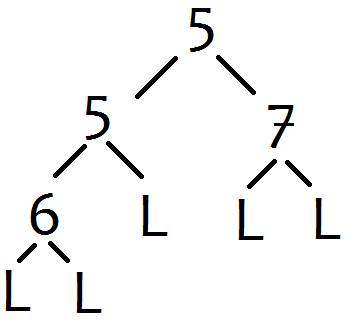
\includegraphics[width=0.2\textwidth]{tree.png}	
\end{block}

\end{frame}




\begin{frame}[fragile]
\frametitle{Towards a more general fold}
\begin{itemize}
\item The recursive structure (in this case Op1 and Op2 child nodes) is specific for each recursive datatype
\item We can define this datatype without recursion as follows
\end{itemize}

\begin{lstlisting}
TreeF v c = Op1 v c c
          | Op2 v c c 
          | Leaf 

someTree :: TreeF Integer (TreeF Integer (TreeF Integer (TreeF v c)))	  
someTree = Op1 4 (Op2 3 (Op1 4 Leaf Leaf) Leaf) Leaf	  
\end{lstlisting}


\begin{itemize}
\item This form is also called the 'pattern functor' of Tree		
\item The return type will grow with the depth of the tree 
\item The goal is to express any tree with a \textit{single type}	
\end{itemize}

\end{frame}


\begin{frame}[fragile]
\frametitle{Fixed point combinator}
\begin{itemize}
\item For the purpose of expressing the TreeF with a single type we can use a datatype fixed point combinator
\item The definition of this combinator is 
\end{itemize}

\begin{lstlisting}
newtype Fix f = In (f (Fix f))

out :: Fix f -> f (Fix f)
out (In x) = x
\end{lstlisting}


\begin{itemize}
\item The combinator closes the type under repeated applications
\item It is analogous to the fixed point equation $x = f (x)$ 	
\item The In and out functions have a structure of a function, that is

\end{itemize}

\begin{lstlisting}
*Main> :t out 
out :: Fix f -> f (Fix f)

*Main> :t In
In :: f (Fix f) -> Fix f
\end{lstlisting}


\end{frame}



\begin{frame}[fragile]
\frametitle{Using the fixed point combinator in Tree}
\begin{itemize}
\item Now to get rid of the repeated applications of TreeF to itself we can apply in to In in the type Fix f
\end{itemize}

\begin{lstlisting}
data TreeF v c = Op1 v c c | Op2 v c c | Leaf

newtype Fix f = In (f (Fix f))
type Tree v = Fix (TreeF v)

exampleTree :: Tree Int
exampleTree = In $ Op1 5 
                    (In $ Op2 5 
                       (In $ Op1 6 (In Leaf) (In Leaf))
                       (In Leaf)) 
                    (In $ Op2 7 (In Leaf) (In Leaf))
\end{lstlisting}


\begin{itemize}
\item We are wrapping the TreeF constructors with an additional In constructor of the Fix datatype
\item We get a single type signature in a function dealing with recursive datatypes
\item For the datatype to be useful we need a way to traverse and evaluate it (fold-like style) 

\end{itemize}

\begin{lstlisting}
*Main> :t out 
out :: Fix f -> f (Fix f)

*Main> :t In
In :: f (Fix f) -> Fix f
\end{lstlisting}


\end{frame}






\begin{frame}[fragile]
\frametitle{TreeF as a functor}
\begin{itemize}
\item fold traverses each element in a list and gives back a single value 
\item In order to evaluate TreeF node we need evaluate it's children
\item We decouple the evaluation of the node itself and the recursive traversal of it's children	
\end{itemize}

\begin{lstlisting}
instance Functor (TreeF v) where
  fmap f Leaf = Leaf
  fmap f (Op1 v l r) = Op1 v (f l) (f r)
  fmap f (Op2 v l r) = Op2 v (f l) (f r)
\end{lstlisting}


\begin{itemize}
\item We make a functor out of TreeF where fmap :: Functor f $ \Rightarrow (a \rightarrow b) \rightarrow$ f a $\rightarrow$ f b
\item If we fmap a function on a TreeF value it will propagate this function through the whole tree 
\end{itemize}

\end{frame}



\begin{frame}[fragile]
\frametitle{Defining an algebra}
\begin{itemize}
\item Now we need to define a function for evaluation the nodes in the tree 
\item We define this function on the TreeF datatype 
\end{itemize}

\begin{lstlisting}
data TreeF v c = Op1 v c c | Op2 v c c | Leaf

intAlg :: TreeF Int Int -> Int
intAlg Leaf = 1
intAlg (Op1 v l r) = v * (l + r)
intAlg (Op2 v l r) = v * (l - r)
\end{lstlisting}


\begin{itemize}
\item In the literature this function is called an algebra
\item An algebra describes how to map a functor where the recursive positions have already been evaluated to a result
\item Notice we have specialized the recursive positions to an Int datatype. This is called a carrier. 	
\item We can use any type as carrier, thus redefining the purpose and calculations in the tree. 	
\end{itemize}

\end{frame}





\begin{frame}[fragile]
\frametitle{Algebra in more detail}
\begin{itemize}
\item What exactly is an algebra? 
\item Let C be a category from the category theory. An algebra of a functor F is a tuple containing an object A (the carrier) in C and a morphism alg:$F(X) \rightarrow X$. 
\item Why was intAlg called an algebra?
\item The type signature was intAlg :: TreeF Int Int $\rightarrow$ Int
\item In plain english it was intAlg :: functor type\_used\_in\_functor carrier\_type $\rightarrow$ carrier\_type
\item In other words it has all the parts an algebra needs: a functor, a carrier and it itself defines a morphism $F(X) \rightarrow X$
\end{itemize}

\end{frame}



\begin{frame}[fragile]
\frametitle{Toward a general fold-like function}
\begin{itemize}
\item So far we have a way to traverse the tree and a way to evaluate each node of the tree.
\item We could already formulate a fold-like function which would collapse the tree into a single value (of the carrier datatype)	
\item The goal is to define a general higher order fold-like function, which would be able to operate on any algebra and functor
\item In order to derive this function, we have to go slightly deeper into the theoretical underpinings of algebra 
\end{itemize}



\end{frame}



\begin{frame}[fragile]
\frametitle{Toward a general fold-like function}
\begin{itemize}
\item If we specify the generalised fold through the algebra and carrier that we defined so far, we would get a function specialised for just that one case
\item we have to use a more 'generic' algebra, one that would also encompass this one	
\item How could we find such an algebra?
\item Recap: Let C be a category from the category theory. An algebra of a functor F is a tuple containing an object A (the carrier) in C and a morphism alg:$F(X) \rightarrow X$. 
\item Hint: we already can hide \textbf{any} functor in the Fix datatype, so it's 'generic' enough
\item Could we somehow use the Fix to create this generalised algebra? What would be the alg morphism and what would be the carrier?
\item If we remember the contructor of Fix (the In function):	
\end{itemize}


\begin{lstlisting}
*Main> :t In
In :: f (Fix f) -> Fix f
\end{lstlisting}


\begin{itemize}
\item We see the resamblance to the morphism $F(X) \rightarrow X$. As Fix is a 'fix point' we have that the carrier would be the Fix datatype
\end{itemize}

\end{frame}









\begin{frame}[fragile]
\frametitle{Pictorial representation of algebras}

\begin{block}{Two algebras}
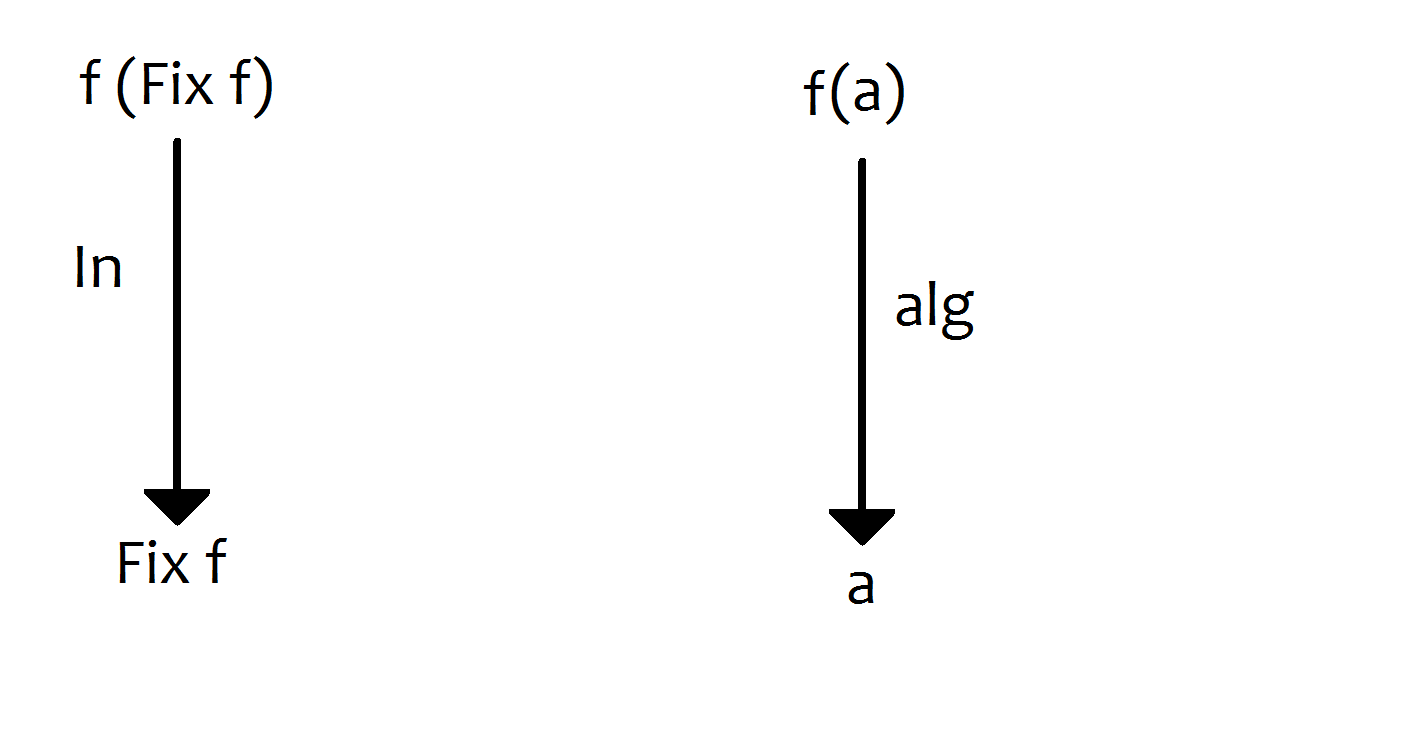
\includegraphics[width=0.8\textwidth]{graf1.png}	
\end{block}
\begin{itemize}
\item We have two separate algebras, the one with Fix and some another which represents any other algebra
\item if we define our general fold on the Fix-Algebra we need a way to map from it to any other algebra.	
\end{itemize}

\end{frame}






\begin{frame}[fragile]
\frametitle{Commutative diagram}

\begin{block}{Unknown mapping}
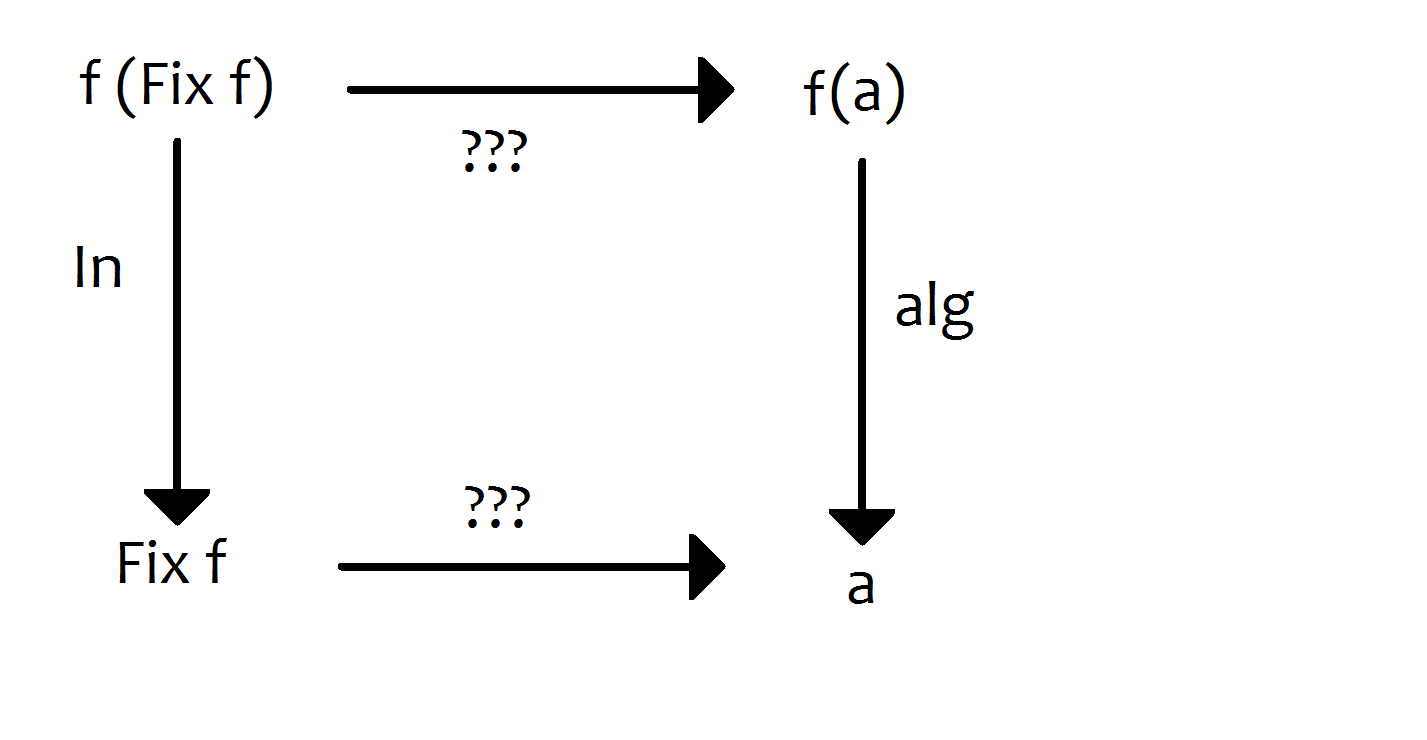
\includegraphics[width=0.8\textwidth]{graf2.png}	
\end{block}
\begin{itemize}
\item We somehow need to define the mapping between these datatype
\end{itemize}

\end{frame}





\begin{frame}[fragile]
\frametitle{Commutative diagram}

\begin{block}{With mapping}
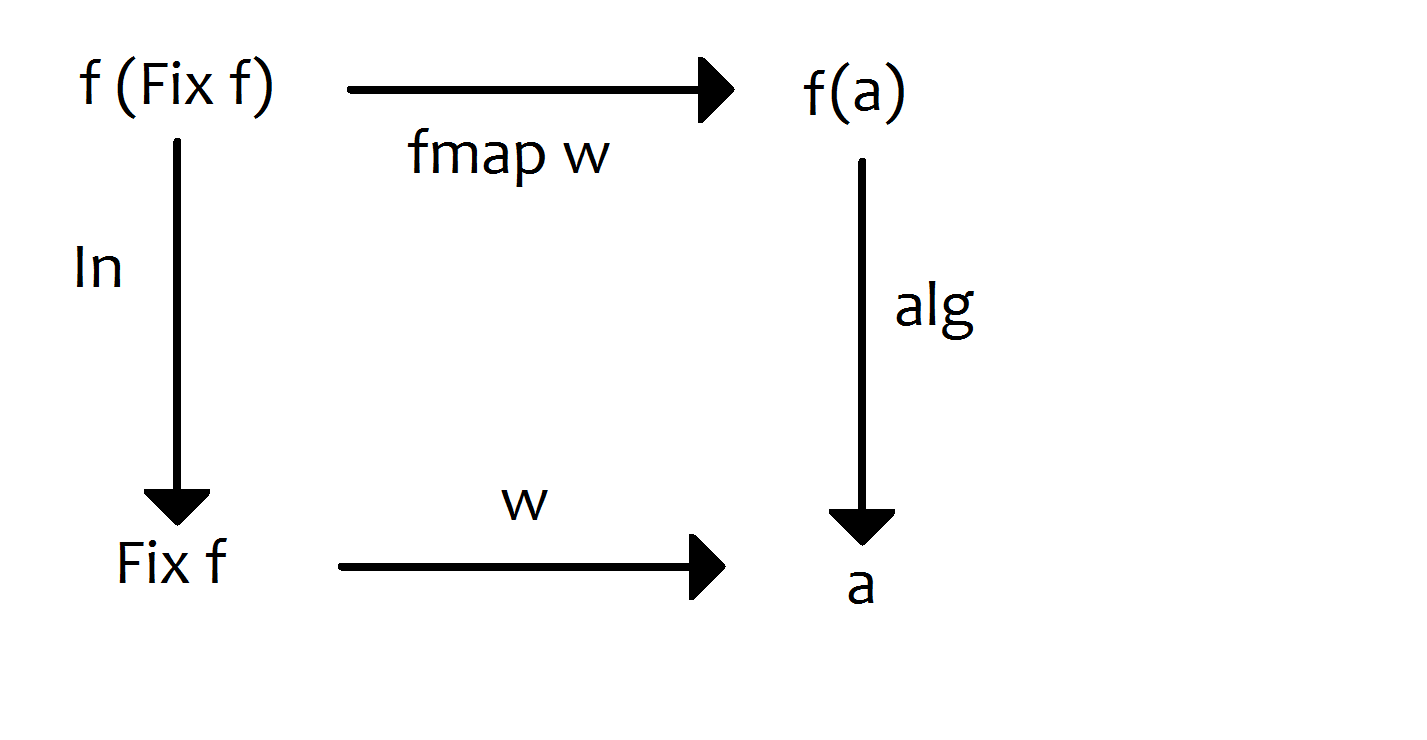
\includegraphics[width=0.8\textwidth]{graf3.png}	
\end{block}
\begin{itemize}
\item We just replaced the questionmarks with w
\item Because f is a functor we can use fmap to apply w to f (Fix f)	
\item How can we find w and somehow incorporate alg so that we can evaluate any algebra? 	
\end{itemize}

\end{frame}





\begin{frame}[fragile]
\frametitle{Commutative diagram}

\begin{block}{Inverting the arrow}
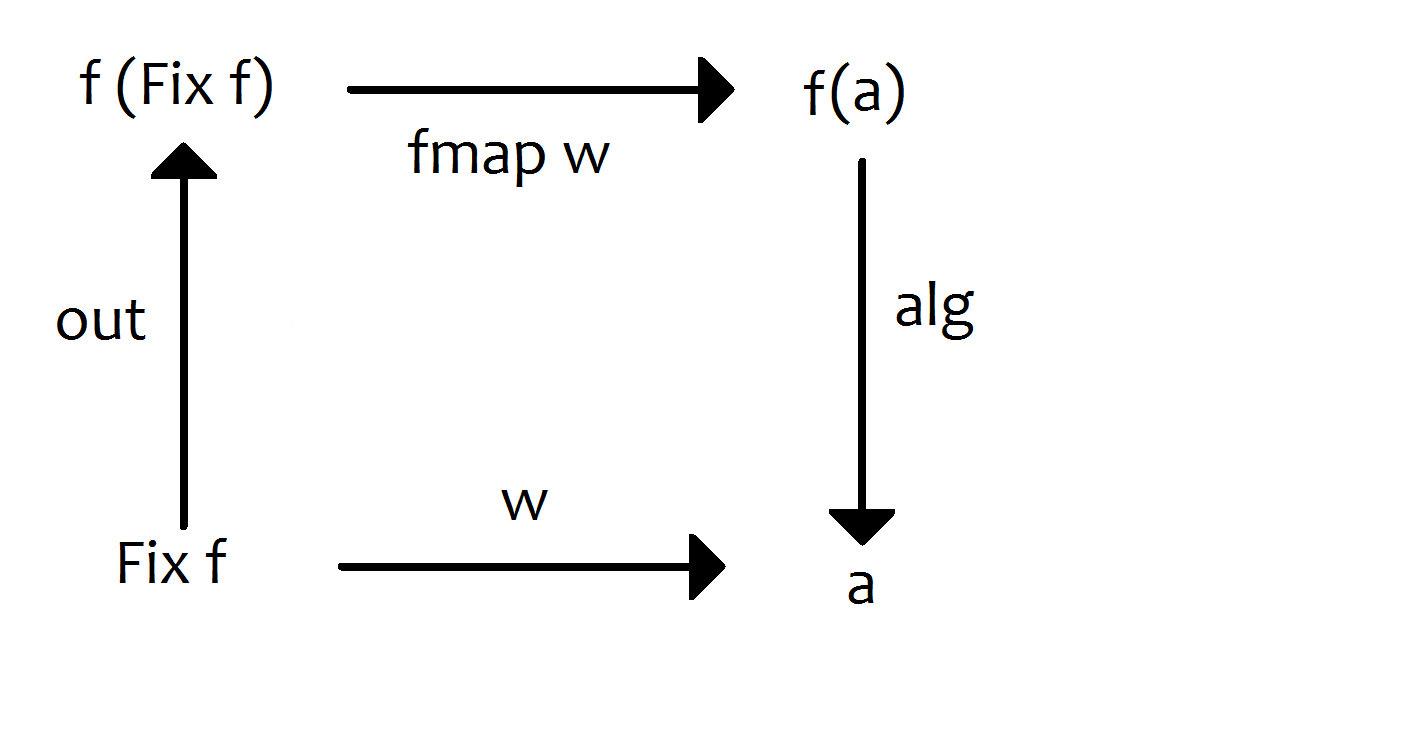
\includegraphics[width=0.8\textwidth]{graf4.png}	
\end{block}
\begin{itemize}
\item There are (at least) 2 tricks! The first is that we invert an arrow and use the out function
\item The second trick is that we define w recursively using itself in the definition	
\end{itemize}

\begin{lstlisting}
w = alg . (fmap w) . out
\end{lstlisting}

\end{frame}




\begin{frame}[fragile]
\frametitle{Defining cata}

\begin{itemize}
\item Why wouldn't the recursive definition loop forever? w calls w in it's body, so it could loop forever. 
\item But since we are using fmap, it peels only a finite sequence of layers in Fix, at some point it will stop
\item The generalised fold is called a catamorphism
\item In order to supply in with a custom alg function, we can turn in into a higher order function	
\end{itemize}

\begin{lstlisting}
cata' =  alg . (fmap cata') . out

cata :: Functor f => (f a -> a) -> Fix f -> a
cata alg = alg . fmap (cata alg) . out
\end{lstlisting}

\end{frame}



\begin{frame}[fragile]
\frametitle{A practical example}

\begin{itemize}
\item We can try the catamorphism on our tree
\end{itemize}

\begin{lstlisting}
cata :: Functor f => (f a -> a) -> Fix f -> a
cata alg = alg . fmap (cata alg) . out

exampleTree :: Tree Int
exampleTree = In $ 
    Op1 5 
      (In $ Op2 5 
         (In $ Op1 6 (In Leaf) (In Leaf))
         (In Leaf)) 
      (In $ Op2 7 (In Leaf) (In Leaf))

intAlg :: TreeF Int Int -> Int
intAlg Leaf = 1
intAlg (Op1 v l r) = v * (l + r)
intAlg (Op2 v l r) = v * (l - r)

print $ cata intAlg exampleTree //265

\end{lstlisting}

\end{frame}







\begin{frame}[fragile]
\frametitle{Properties}

\begin{block}{catamorphism}
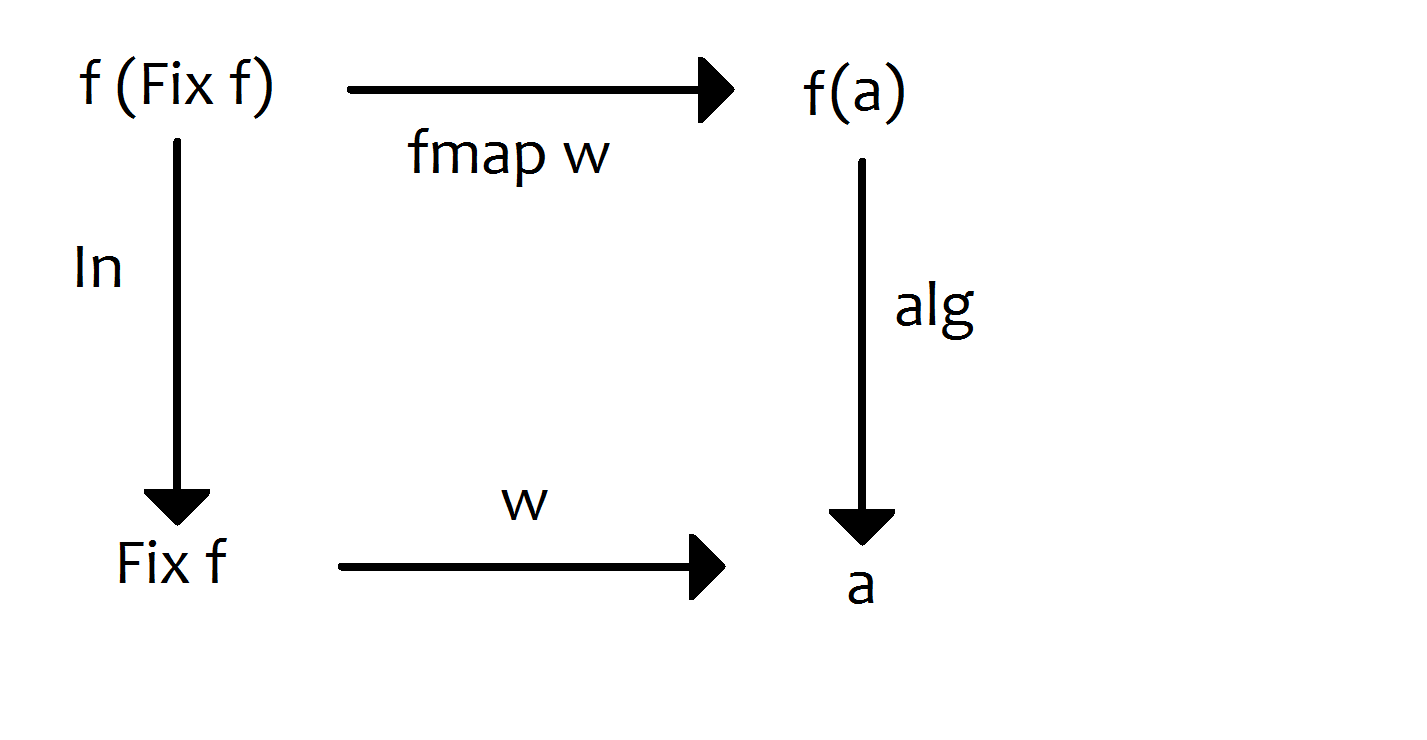
\includegraphics[width=0.2\textwidth]{graf3.png}	
\end{block}
\begin{itemize}
\item Catamorphisms have the same laws as folds. As to avoid introducing new mathematical concepts I only mention the 
	spirit of the laws without regard to the exactness of the formulation 
\item The universality property translated to the diagram above would state that

\end{itemize}

\begin{lstlisting}
alg . (fmap w) = w . In
\end{lstlisting}

\begin{itemize}
	\item The fusion law states that the composition of a function and a catamorphism can be rewritten as a catamorphism (no need for intermediate data representations).
\end{itemize}

\begin{lstlisting}
h . w = w'
\end{lstlisting}

\begin{itemize}
\item When we have 2 algebras in the same functor with a different carrier then using the Banana Split Law 2 catamorphisms can be expressed as a single catamorphism (single traversal of the datatype)
\end{itemize}
\end{frame}



\begin{frame}[fragile]
\frametitle{Limitations}

\begin{itemize}
\item Catamorphisms are part of the datatype generic approch to programming 
\item Generic functions can be used to write serialisers [2], evaluators, pretty-printers ... 
\item The approach deals with datatypes with regular structure.
\item Different methods have to be used to deal with non-regular datatypes (nested or mutually recursive datatypes) 	
\item Example of a nested datatype:	
\end{itemize}

\begin{lstlisting}
data Nest a = Nil | Cons (a, Nest (a, a))

Cons 
   (10,
      Cons 
        ((10,10),
          Cons 
             (((10,10),(10,10)),
                  Nil)))
\end{lstlisting}

\end{frame}




\begin{frame}[fragile]
\frametitle{Related topics}

\begin{itemize}
\item Paramorphism is an extension of catamorphism
\item Paramorphism operate on the results of the evaluation of substructures as well as on substructures themselves	
\item Usefull when you need to further examine the data from which the result was computed	
\item We could define a monadic catamorphism where the algebra is alg : f a $\rightarrow$ m a where m is a monad 
\item The benefit is that the we can use monads in the algebra but don't have to specify the monads in the pattern functor
\item We can use memoization in catamorphism (define a memoizing catamorphism) to speed up computations
\end{itemize}

\end{frame}


\begin{frame}[fragile]
\frametitle{Size Matters}

\begin{itemize}
\item Smaller code bases have fewer bugs
\item Therefore it is advantageous to strive for less code
\item There are to trends related to project size	
\item 1. Concision (syntax, convention over configuration ..), which leads to small improvements
\item 2. Generality (leads to big improvements) 
\item The difference of solving problems more \textbf{efficiently} vs. solving problems \textbf{differently}   
\end{itemize}

\end{frame}





\begin{frame}[fragile]
\frametitle{References}

\begin{itemize}
\item [1] A tutorial on the universality and expressiveness of fold, Graham Hutton, 1999
\item [2] Generic Storage in Haskell, Sebastiaan Visser, Andres Löh, 2010
\item [3] When is a function a fold or an unfold?, Jeremy Gibbons, Graham Hutton, Thorsten Altenkirch, 2001
\item [4] Understanding F-Algebras, blog post on www.fpcomplete.com, Bartosz Milewski, 2013
\item [5] Catamorphisms, blog post on www.fpcomplete.com, Edward Kmett, 2014
\item [6] Initial Algebra Semantics is Enough!, Patricia Johann, Neil Ghani, 2007
\item [7] Functional Programming with Bananas, Lenses, Envelopes and Barbed Wire, Erik Meijer Maarten Fokkinga, Ross Paterson, 1991
\end{itemize}

\end{frame}




\begin{frame}[fragile]
\frametitle{}

\begin{itemize}
\item Questions?
\end{itemize}

\begin{block}{Recursive giraffe, Farley Katz cartoon }
\includegraphics[width=0.6\textwidth]{giraffe.jpg}	
\end{block}
\end{frame}










\end{document}
